\documentclass{beamer}
\usetheme{Madrid}
\usecolortheme{default}

\usepackage{tikz}
\usetikzlibrary{arrows.meta, positioning, fit}
\usepackage{graphicx}

\title[Edge Device Gateway]{A Unified Driver--Compute Framework for\\General-Purpose Computation on Edge Devices}
\subtitle{A Case Study in Biomedical Sensing}
\author{%
  \begin{tabular}[t]{c}Kommana Sri Krishna Ramesh\\[2pt]\footnotesize 23ECB0B19\end{tabular}
  \and
  \begin{tabular}[t]{c}Bibek Chaudhary\\[2pt]\footnotesize 23ECB0F33\end{tabular}
  \and
  \begin{tabular}[t]{c}Abhinav Magesh\\[2pt]\footnotesize 23ECB0F25\end{tabular}
}
\institute{Team B19}
\date{\today}

\begin{document}

\frame{\titlepage}

\begin{frame}{Motivation}
\begin{itemize}
  \item Biomedical edge devices are siloed: pulse oximeters, ECG monitors, BP cuffs,
    glucometers each use a different transport and data format.
  \item Serial (USB), Bluetooth Low Energy (BLE GATT), proprietary USB -- no common interface.
  \item Integrating each device today means writing a bespoke driver \emph{and} a bespoke
    pipeline every time.
  \item \textbf{Goal:} one general software framework that can connect to \emph{any} edge
    device and compute \emph{anything} on its data.
\end{itemize}
\end{frame}

\begin{frame}{Problem Statement}
Given devices $D=\{d_1,\dots,d_n\}$ over transports $T(d_i)\in\{\text{serial},\text{BLE},\text{USB}\}$
emitting readings $(t, \text{channel}, \text{value})$, build a system where:
\begin{itemize}
  \item Adding a \textbf{new device} = implementing one driver interface, no other changes.
  \item Adding a \textbf{new computation} = implementing one compute-module interface, no
    driver changes.
  \item The system is \textbf{always demonstrable}, even with zero hardware attached.
\end{itemize}
\end{frame}

\begin{frame}{Related Work}
\begin{itemize}
  \item \textbf{IEEE 11073 / Bluetooth GATT health profiles} -- standardize data \emph{within}
    a device class, not across heterogeneous classes/transports.
  \item \textbf{EdgeX Foundry, Node-RED} -- general IoT gateway platforms, but need separate
    server infrastructure.
  \item \textbf{WebSerial / Web Bluetooth / WebUSB} -- browser APIs for direct hardware access;
    underused as a \emph{general-purpose} device integration layer. We treat the browser tab
    itself as a universal, zero-install gateway.
\end{itemize}
\end{frame}

\begin{frame}{Proposed Architecture}
\begin{center}
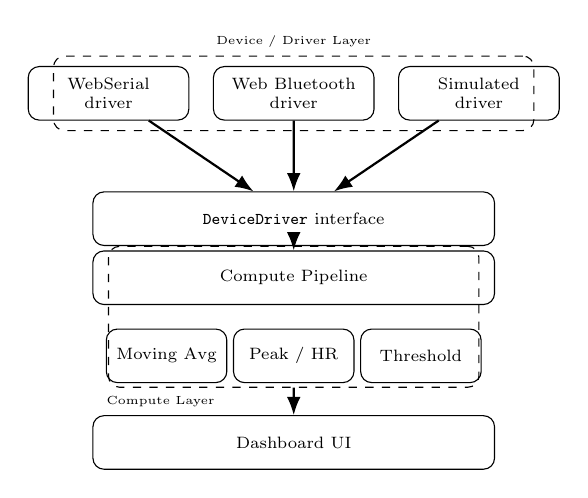
\begin{tikzpicture}[
  box/.style={draw, rounded corners, align=center, minimum width=2.4cm, minimum height=0.8cm, font=\scriptsize},
  layer/.style={draw, dashed, rounded corners, inner sep=6pt},
  arr/.style={-{Latex}, thick},
  scale=0.85, every node/.style={scale=0.85}
]
\node[box] (serial) {WebSerial\\driver};
\node[box, right=0.3cm of serial] (ble) {Web Bluetooth\\driver};
\node[box, right=0.3cm of ble] (sim) {Simulated\\driver};
\node[layer, fit=(serial)(ble)(sim), label={[font=\tiny]above:Device / Driver Layer}] (devicelayer) {};

\node[box, below=0.9cm of ble, minimum width=6cm] (iface) {\texttt{DeviceDriver} interface};

\node[box, below=0.8cm of ble, yshift=-1.0cm, minimum width=6cm] (pipeline) {Compute Pipeline};
\node[box, below=0.3cm of pipeline, xshift=-1.9cm, minimum width=1.8cm] (mavg) {Moving Avg};
\node[box, below=0.3cm of pipeline, minimum width=1.8cm] (peak) {Peak / HR};
\node[box, below=0.3cm of pipeline, xshift=1.9cm, minimum width=1.8cm] (thresh) {Threshold};
\node[layer, fit=(pipeline)(mavg)(peak)(thresh), label={[font=\tiny]below left:Compute Layer}] (complayer) {};

\node[box, below=1.4cm of pipeline, minimum width=6cm] (ui) {Dashboard UI};

\draw[arr] (serial) -- (iface);
\draw[arr] (ble) -- (iface);
\draw[arr] (sim) -- (iface);
\draw[arr] (iface) -- (pipeline);
\draw[arr] (complayer) -- (ui);
\end{tikzpicture}
\end{center}
\end{frame}

\begin{frame}{The \texttt{DeviceDriver} Interface}
Every device integration implements the same contract:
\begin{itemize}
  \item \texttt{isSupported()} -- browser/hardware capability check
  \item \texttt{connect()} / \texttt{disconnect()}
  \item \texttt{getStatus()} -- disconnected / connecting / connected / error
  \item \texttt{onData(callback)} -- stream of \texttt{\{timestamp, channel, value, unit\}}
\end{itemize}
\vspace{0.3cm}
The dashboard only ever talks to this interface -- it never knows whether data is coming from
real hardware or the simulator.
\end{frame}

\begin{frame}{Three Driver Types Built}
\begin{itemize}
  \item \textbf{WebSerial driver} -- generic USB-serial device, line-delimited
    \texttt{channel,value} readings.
  \item \textbf{Web Bluetooth driver} -- standard BLE \textbf{Heart Rate Service (0x180D)},
    works with real commercial BLE straps/watches.
  \item \textbf{Simulated driver} -- synthetic ECG / SpO\textsubscript{2} / HR / BP generator
    with selectable scenarios (normal, tachycardia, desaturation). Always available, default
    on load -- the demo never dead-ends.
\end{itemize}
\end{frame}

\begin{frame}{Compute Pipeline Concept}
\begin{itemize}
  \item Every incoming reading, from \emph{any} driver, is fanned through an ordered list of
    pluggable \texttt{ComputeModule}s.
  \item A module can emit \textbf{derived readings} (e.g. a filtered value, a computed heart
    rate) and/or \textbf{alert events}.
  \item Modules can be enabled/disabled and configured live from the dashboard.
\end{itemize}
\end{frame}

\begin{frame}{Compute Modules Built}
\begin{itemize}
  \item \textbf{Moving-average filter} -- smooths a noisy channel (e.g. SpO\textsubscript{2}).
  \item \textbf{ECG peak / heart-rate detector} -- threshold-crossing R-peak detection with a
    refractory period; derives instantaneous BPM live from the raw waveform.
  \item \textbf{Threshold alerting} -- configurable per-channel warning/critical thresholds;
    emits alerts on severity transitions (no duplicate spam).
\end{itemize}
\end{frame}

\begin{frame}{Dashboard: Connect}
\begin{center}
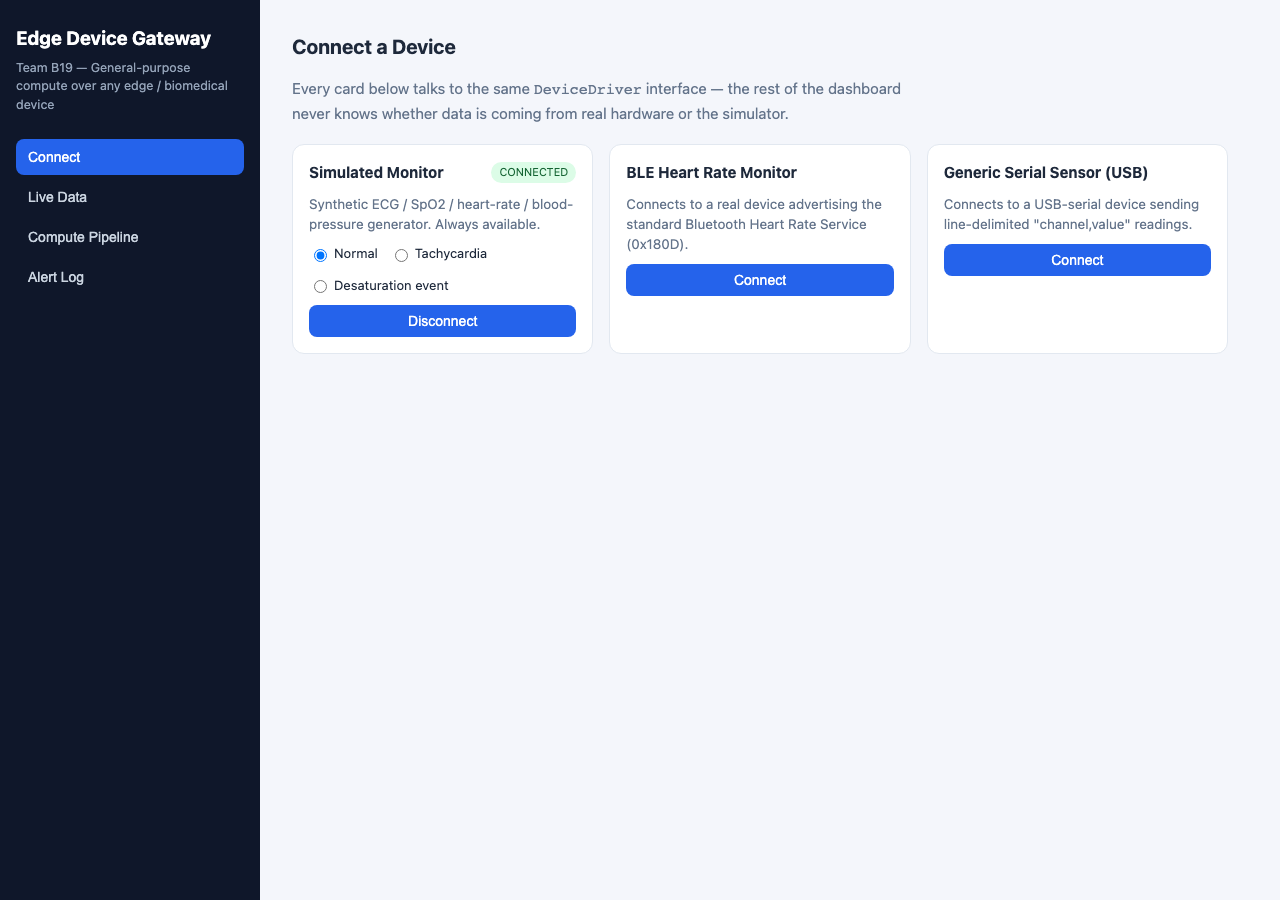
\includegraphics[width=0.95\textwidth]{figures/connect-panel.png}
\end{center}
\end{frame}

\begin{frame}{Dashboard: Live Data}
\begin{center}
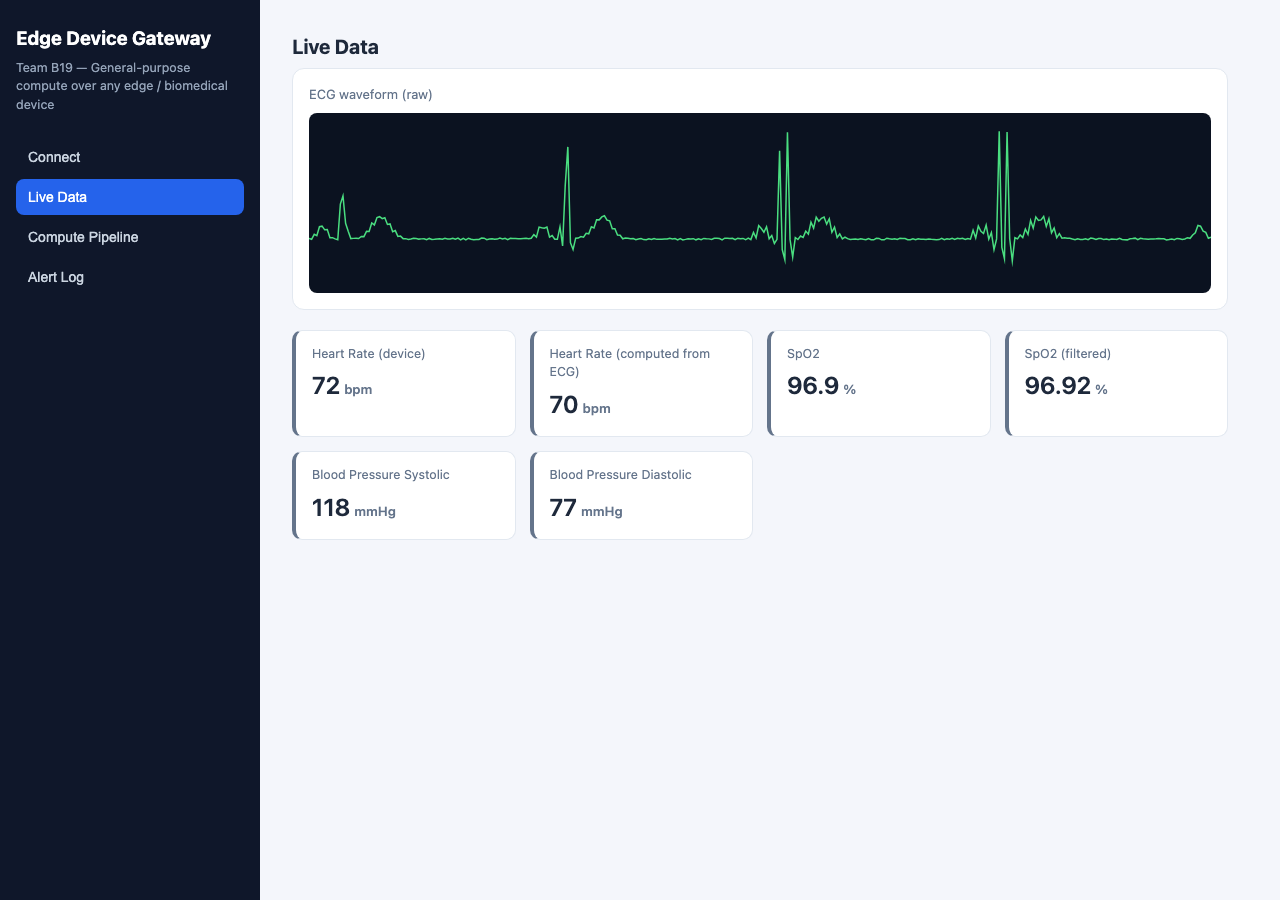
\includegraphics[width=0.95\textwidth]{figures/live-data-panel.png}
\end{center}
\end{frame}

\begin{frame}{Dashboard: Compute Pipeline}
\begin{center}
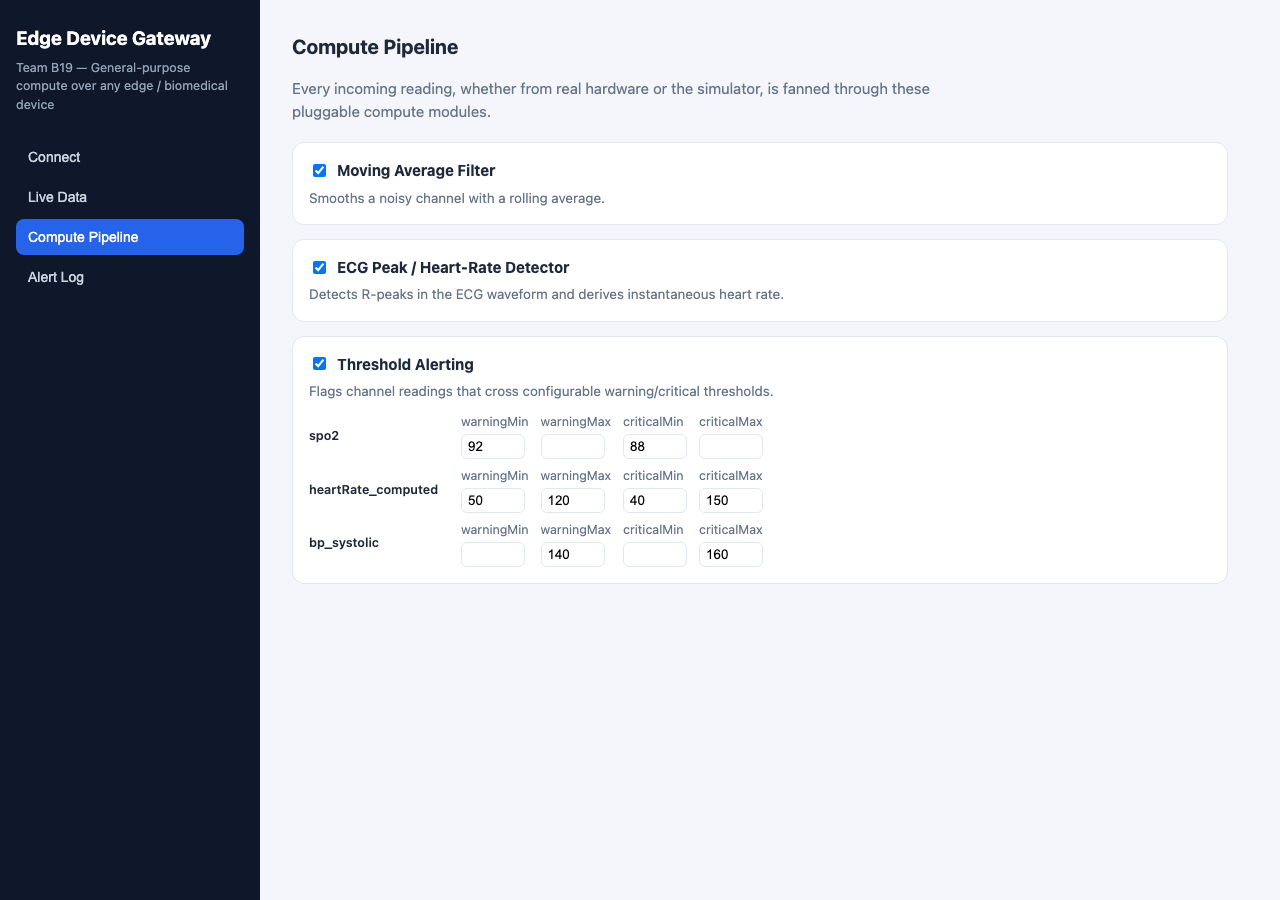
\includegraphics[width=0.95\textwidth]{figures/pipeline-panel.png}
\end{center}
\end{frame}

\begin{frame}{Dashboard: Alert Log}
\begin{center}
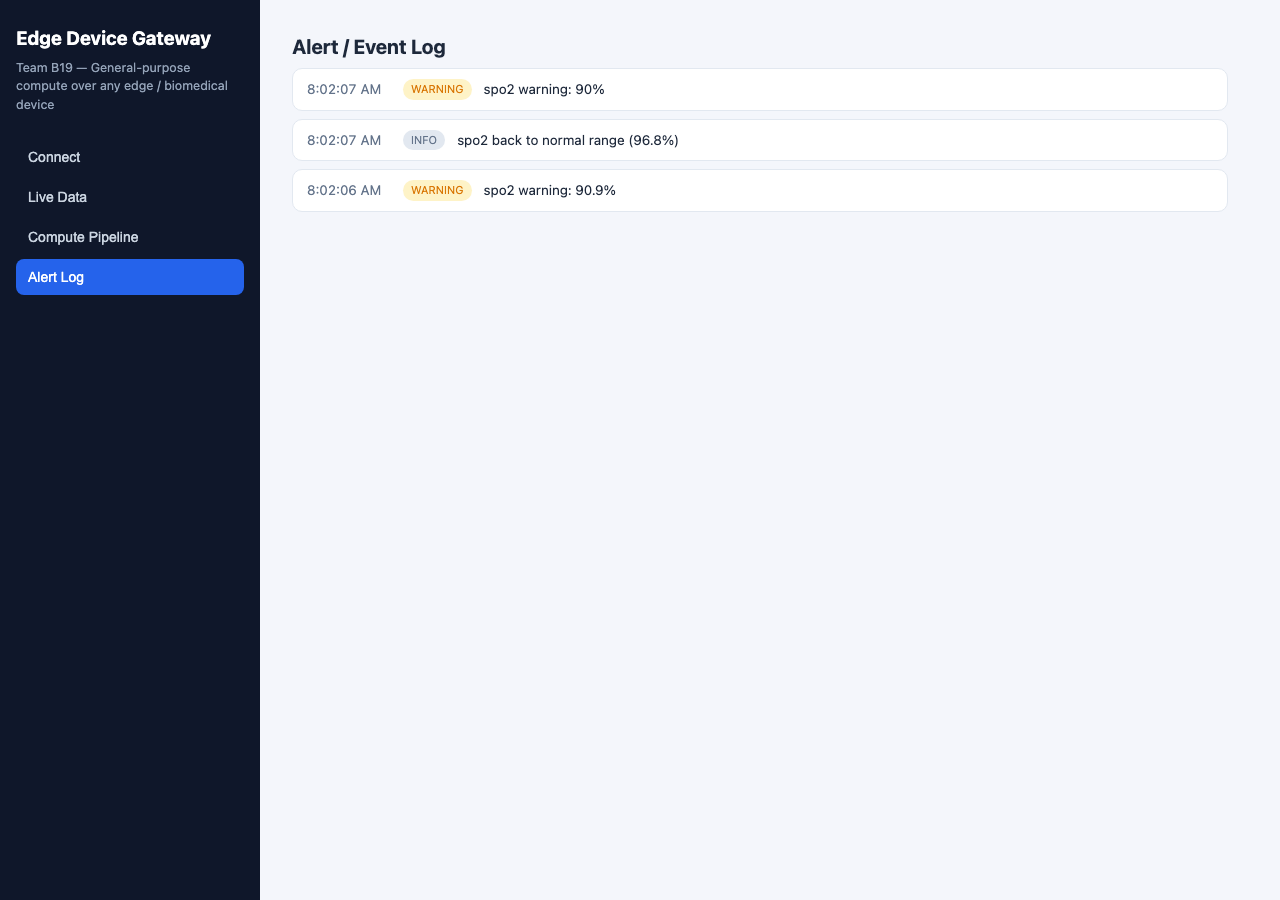
\includegraphics[width=0.95\textwidth]{figures/alert-log.png}
\end{center}
\end{frame}

\begin{frame}{Use Case Walkthrough}
\begin{enumerate}
  \item Simulated monitor connects automatically -- live ECG, SpO\textsubscript{2}, HR, BP.
  \item Switch scenario to \textbf{Desaturation event}.
  \item Moving-average filter smooths the noisy SpO\textsubscript{2} channel.
  \item SpO\textsubscript{2} crosses the warning threshold (92\%) $\rightarrow$ alert logged.
  \item Same pipeline, zero code changes, would fire identically on a real pulse oximeter.
\end{enumerate}
\end{frame}

\begin{frame}{Extensibility \& Future Work}
\begin{itemize}
  \item \textbf{WebUSB driver} -- interface already accommodates it; deferred as lower priority.
  \item \textbf{Clinical-grade signal processing} -- e.g. Pan--Tompkins QRS detection.
  \item \textbf{Persistence \& multi-device trends} -- optional storage layer.
  \item \textbf{Native companion apps} -- for browsers without WebSerial/Web Bluetooth.
\end{itemize}
\end{frame}

\begin{frame}{Conclusion}
\begin{itemize}
  \item A driver--compute architecture generalizes edge device integration: transport-specific
    acquisition, transport-agnostic computation.
  \item Validated with a working, client-only prototype connecting to \emph{real} hardware
    (WebSerial, Web Bluetooth) and a simulator, with zero backend.
  \item New device = one driver. New analysis = one compute module. Independently.
\end{itemize}
\end{frame}

\begin{frame}{Team B19}
\begin{itemize}
  \item Kommana Sri Krishna Ramesh -- 23ECB0B19
  \item Bibek Chaudhary -- 23ECB0F33
  \item Abhinav Magesh -- 23ECB0F25
\end{itemize}
\vspace{0.5cm}
\centering \Large Thank you
\end{frame}

\end{document}
